\documentclass[
11pt, % The default document font size, options: 10pt, 11pt, 12pt
%codirector, % Uncomment to add a codirector to the title page
]{charter} 

\usepackage{pdflscape}

% El títulos de la memoria, se usa en la carátula y se puede usar el cualquier lugar del documento con el comando \ttitle
\titulo{Detección de patologías cardiopulmonares mediante redes neuronales aplicadas a señales de auscultación} 

% Nombre del posgrado, se usa en la carátula y se puede usar el cualquier lugar del documento con el comando \degreename
\posgrado{Carrera de Especialización en Inteligencia Artificial}

% Tu nombre, se puede usar el cualquier lugar del documento con el comando \authorname
% IMPORTANTE: no omitir titulaciones ni tildación en los nombres, también se recomienda escribir los nombres completos (tal cual los tienen en su documento)
\autor{Ing. Santiago Federico Bettig}

% El nombre del director y co-director, se puede usar el cualquier lugar del documento con el comando \supname y \cosupname y \pertesupname y \pertecosupname
\director{Dr. Ing. Leandro Javier Cymberknop}
\pertenenciaDirector{CIBIO, UTN FRBA} 
\codirector{} % para que aparezca en la portada se debe descomentar la opción codirector en los parámetros de documentclass
\pertenenciaCoDirector{FIUBA}

% Nombre del cliente, quien va a aprobar los resultados del proyecto, se puede usar con el comando \clientename y \empclientename
\cliente{Dra. Laura Méndez}
\empresaCliente{CIBIO, UTN FRBA}
 
\fechaINICIO{28 de abril de 2026}		%Fecha de inicio de la cursada de GdP \fechaInicioName
\fechaFINALPlan{16 de junio de 2026} 	%Fecha de final de cursada de GdP
\fechaFINALTrabajo{diciembre de 2026}	%Fecha de defensa pública del trabajo final


\begin{document}

\maketitle
\thispagestyle{empty}
\pagebreak


\thispagestyle{empty}
{\setlength{\parskip}{0pt}
\tableofcontents{}
}
\pagebreak


\section*{Registros de cambios}
\label{sec:registro}


\begin{table}[ht]
\label{tab:registro}
\centering
\begin{tabularx}{\linewidth}{@{}|c|X|c|@{}}
\hline
\rowcolor[HTML]{C0C0C0} 
Revisión & \multicolumn{1}{c|}{\cellcolor[HTML]{C0C0C0}Detalles de los cambios realizados} & Fecha      \\ \hline
0      & Creación del documento                                 &\fechaInicioName \\ \hline
1      & Se completa hasta el punto 5 inclusive                 & {09} de {mayo} de 2026 \\ \hline
2      & Se completa hasta el punto 9 inclusive                 & {17} de {mayo} de 2026 \\ \hline
3      & Se completa hasta el punto 12 inclusive                & {23} de {mayo} de 2026 \\ \hline
4      & Se completa el plan	                                  & {30} de {mayo} de 2026 \\ \hline
5      & Correcciones menores	                                  & {07} de {junio} de 2026 \\ \hline
6      & Correcciones menores	                                  & {08} de {junio} de 2026 \\ \hline

% Si hay más correcciones pasada la versión 4 también se deben especificar acá

\end{tabularx}
\end{table}

\pagebreak

\section*{Acta de constitución del proyecto}
\label{sec:acta}

\begin{flushright}
Buenos Aires, \fechaInicioName
\end{flushright}

\vspace{2cm}

Por medio de la presente se acuerda con el \authorname\hspace{1px} que su Trabajo Final de la
\degreename\hspace{1px} se titulará ``\ttitle'' y consistirá en desarrollar un sistema de clasificación
automática de patologías cardiopulmonares mediante redes neuronales convolucionales aplicadas a señales 
de auscultación. El trabajo tendrá un presupuesto preliminar estimado de 450 horas 
y un costo estimado de \$ 5.875.000, con fecha de inicio el \fechaInicioName\hspace{1px} 
y fecha de presentación pública en \fechaFinalName.

Se adjunta a esta acta la planificación inicial.

\vfill

% Esta parte se construye sola con la información que hayan cargado en el preámbulo del documento y no debe modificarla
\begin{table}[ht]
\centering
\begin{tabular}{ccc}
\begin{tabular}[c]{@{}c@{}}Dr. Ing. Ariel Lutenberg \\ Director posgrado FIUBA\end{tabular} & \hspace{2cm} & \begin{tabular}[c]{@{}c@{}}\clientename \\ \empclientename \end{tabular} \vspace{2.5cm} \\ 
\multicolumn{3}{c}{\begin{tabular}[c]{@{}c@{}} \supname \\ Director del Trabajo Final\end{tabular}} \vspace{2.5cm} \\
\end{tabular}
\end{table}

\vspace{100px}
\section{1. Descripción técnica-conceptual del proyecto a realizar}
\label{sec:descripcion}

\subsection{Contexto del proyecto}
Las enfermedades cardiovasculares y respiratorias representan dos de las principales causas de mortalidad a nivel mundial. 
Según la Organización Mundial de la Salud, las enfermedades cardíacas son responsables de aproximadamente 17 millones de muertes anuales, 
mientras que las enfermedades respiratorias afectan a más de 500 millones de personas. En ambos casos, el diagnóstico temprano 
es determinante para el pronóstico del paciente y para la reducción de costos en el sistema de salud. Sin embargo, acceder a ese diagnóstico 
es un desafío en gran parte del mundo.

\subsection{Problema que se atiende}
La auscultación con estetoscopio es una de las herramientas de diagnóstico más antiguas y vigentes de la medicina clínica.
Permite detectar anomalías en los sonidos del corazón y los pulmones (soplos, arritmias, sibilancias, crepitantes) que son indicativas de patologías graves. 
Es una técnica no invasiva y de bajo costo. Un limitante del método es que su precisión depende, en gran medida, de la experiencia y el entrenamiento del profesional.

Esta limitación resulta crítica en regiones con escasez de especialistas, situación común en buena parte de América Latina. 
Usualmente, es el médico general quien debe interpretar los sonidos cardiopulmonares y decidir si derivar o no al paciente, sin contar 
con el criterio afinado de un cardiólogo o neumólogo. Esta brecha de acceso tiene consecuencias directas en la detección tardía de enfermedades tratables.

\subsection{Estado del arte}
En los últimos años, el aprendizaje profundo permitió desarrollar nuevas técnicas y aplicaciones para el análisis de señales biomédicas.
La pandemia de COVID-19 aceleró el interés por herramientas de diagnóstico remoto y automatizado, lo que impulsó el desarrollo de sistemas capaces 
de analizar sonidos respiratorios y cardíacos con alta precisión. Distintos desafíos públicos referentes al tema captaron la atención de equipos 
de todo el mundo, los cuales comenzaron a desarrollar algoritmos de clasificación y diagnóstico, lo que generó una amplia literatura en la cual apoyarse.

Los enfoques más exitosos transforman las señales de audio en representaciones tiempo-frecuencia y las procesan con redes neuronales 
convolucionales (CNN), que aprenden automáticamente los patrones acústicos relevantes para cada patología. Algunos trabajos más recientes incorporan 
arquitecturas híbridas o mecanismos de atención que mejoran aún más la precisión. No obstante, la gran mayoría de estos sistemas aborda los sonidos 
cardíacos y pulmonares de forma aislada, como si fueran dominios independientes, cuando en la práctica clínica el médico los evalúa de manera integrada.

\subsection{Solución planteada y propuesta de valor}
Este trabajo propone desarrollar un sistema de clasificación automática de patologías cardiopulmonares que procese señales de auscultación 
mediante redes neuronales convolucionales y abordar conjuntamente los sonidos cardíacos y pulmonares en un único pipeline, como se observa en la figura 1. 
Esta integración representa el principal aporte diferencial respecto al estado del arte: la mayoría de los sistemas existentes tratan ambos dominios 
por separado, mientras que la auscultación clínica real no hace esa distinción.

El proyecto se enmarca en la Especialización en Inteligencia Artificial y se desarrolla en colaboración con el CIBIO (Centro de Investigación y 
Desarrollo en Ingeniería Biomédica) de la UTN Buenos Aires, bajo la dirección de Leandro Cymberknop. Los resultados serán de carácter académico y 
de acceso abierto, para que el CIBIO pueda incorporarlos en líneas de investigación clínica futuras.

El adoptante principal de esta solución es el médico general. Este perfil no necesita un sistema que reemplace 
su criterio clínico, sino uno que lo asista con una segunda opinión objetiva, reproducible y disponible en cualquier entorno donde haya un estetoscopio digital.
La innovación pasa por facilitar el acceso a un nivel de análisis que hoy solo está disponible para quienes tienen acceso a especialistas.
En términos del ciclo de vida, la solución se encuentra en etapa de investigación y prueba de concepto, con foco en la validación técnica del modelo 
sobre datasets públicos de referencia.

\begin{figure}[htpb]
\centering 
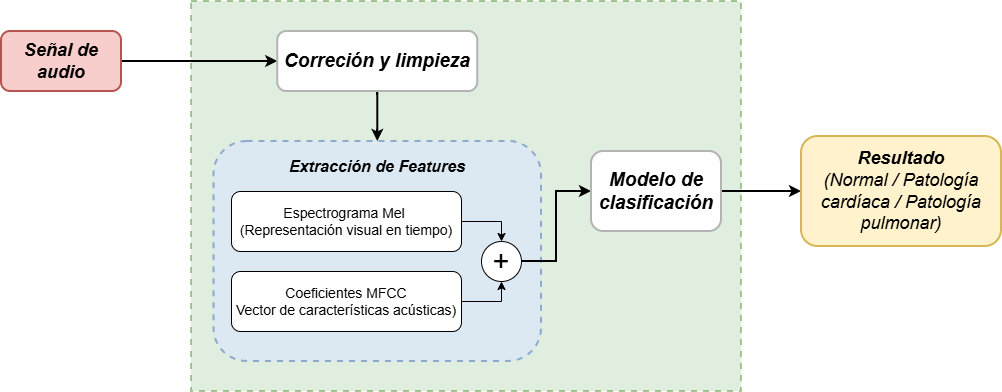
\includegraphics[width=1.0\textwidth]{./Figuras/diagrama_en_bloques.png}
\caption{Diagrama en bloques del proyecto}
\label{fig:diagBloques}
\end{figure}

\vspace{200px}

\section{2. Identificación y análisis de los interesados}
\label{sec:interesados}

\begin{table}[ht]
\begin{tabularx}{\linewidth}{@{}|l|X|X|X|@{}}
\hline
\rowcolor[HTML]{C0C0C0} 
Rol           & Nombre y Apellido & Organización 	  & Puesto 	                                                            \\ \hline
Cliente       & \clientename      & \empclientename	& Referente biomédica de CIBIO                                        \\ \hline
Responsable   & \authorname       & FIUBA        	  & Alumno 	                                                            \\ \hline
Orientador    & \supname          & \pertesupname   & Director de CIBIO                                                   \\ \hline
Usuario final & Médicos generalistas y especialistas & Instituciones de salud & Usuarios potenciales del sistema de apoyo \\ \hline
\end{tabularx}
\end{table}

\begin{itemize}
	\item Responsable: el \authorname\hspace{1px} es desarrollador de firmware hace más de 5 años, con experiencia en 
	procesamiento digital de señales. Previamente trabajó en proyectos de aplicación en el campo de la medicina. Actualmente cursa
	la Carrera de Especialización en Inteligencia Artificial (CEIA). 
	\item Cliente: la \clientename\hspace{1px} es médica especialista y referente biomédica encargada de validar los resultados en el CIBIO.
	\item Orientador: el \supname\hspace{1px} es investigador categoría A en la UTN FRBA y director del grupo de investigación CIBIO. A lo largo de
	su carrera ha realizado numerosos posgrados relacionados con la medicina y la inteligencia artificial. También se desempeña
	como docente de la materia Análisis de Señales y Sistemas (ASyS) en la UTN FRBA.
\end{itemize}

\section{3. Propósito del proyecto}
\label{sec:proposito}

El propósito del proyecto es desarrollar una herramienta de apoyo al diagnóstico médico basada en inteligencia artificial, 
capaz de analizar y clasificar sonidos cardíacos y pulmonares obtenidos mediante un estetoscopio digital. 

La iniciativa busca reducir la dependencia subjetiva del profesional a la interpretación de señales de auscultación,
que ofrezca una segunda opinión objetiva y reproducible que pueda complementar la evaluación clínica. A diferencia de la mayoría de 
los sistemas existentes, que abordan los sonidos cardíacos y pulmonares de forma separada, este trabajo propone un enfoque integrado, 
más cercano a la práctica clínica real.

El proyecto es relevante en contextos con acceso limitado a especialistas, donde una herramienta de este tipo podría 
contribuir a mejorar la detección temprana de enfermedades y disminuir el tiempo en el que el paciente obtenga un diagnóstico certero.

Es importante mencionar que el proyecto busca ser una herramienta de apoyo para el profesional y este debe usarla para brindar el 
mejor diagnóstico posible. El resultado obtenido no deberá ser considerado como un diagnóstico final.

\section{4. Alcance del proyecto}
\label{sec:alcance}

El proyecto incluye:
\begin{itemize}
	\item La recopilación y preprocesamiento de datos de audio provenientes de datasets públicos.
	\item La extracción de features a partir de las señales de auscultación, mediante espectrogramas Mel y coeficientes MFCC.
	\item El diseño, entrenamiento y validación de un modelo de clasificación basado en redes neuronales convolucionales (CNN).
	\item La evaluación del rendimiento del modelo mediante métricas estándar (accuracy, F1-score, matriz de confusión).
		\end{itemize}

El proyecto no incluye:
\begin{itemize}
	\item El desarrollo de hardware ni la integración con un estetoscopio digital físico.
	\item La validación clínica del sistema con pacientes reales ni la obtención de aprobación regulatoria.
	\item El despliegue del modelo en un entorno de producción o aplicación médica real.
	\item La generación de un diagnóstico definitivo; el sistema actúa exclusivamente como herramienta de apoyo y no reemplaza el 
	criterio del profesional de la salud.
\end{itemize}

\section{5. Supuestos del proyecto}
\label{sec:supuestos}

Para el desarrollo del presente proyecto se supone que:

\begin{itemize}
	\item El responsable contará con el tiempo extralaboral suficiente para cumplir con el ciclo de vida del proyecto. Se deben tener en cuenta
	las	responsabilidades y obligaciones extracurriculares.
	\item Se asume que se cuenta con los recursos económicos necesarios para llevar a cabo el proyecto, especificados previamente 
	en el acta de constitución del proyecto.
	\item Los datasets serán accesibles y acordes para la realización del proyecto. No se espera que puedan utilizarse directamente, sino que
	se asume que debe trabajarse previamente sobre los mismos.
	\item Se contará con el equipo (hardware) acorde para el procesamiento de los datos y para la implementación del modelo final.
	\item Se supone que el director del Trabajo Final brindará orientación técnica y metodológica durante el desarrollo del proyecto, 
  de acuerdo con su disponibilidad.
  \item En el caso de que el director no pueda responder las consultas por falta de conocimiento, se acudirá a la persona pertinente dentro 
  del grupo de investigación.
\end{itemize}

\section{6. Product Backlog}
\label{sec:backlog}

Para cada historia de usuario se determina su dificultad, complejidad e incertidumbre.
Su estimación en Story Points (SP) se calcula como la suma de estos tres componentes y se redondea al siguiente valor de la serie de Fibonacci.
\begin{itemize}
  \item Épica 1: exploración y visualización preliminar de datos
    \begin{itemize}
      \item HU1: Como desarrollador, quiero analizar la distribución de datos para identificar desbalances 
      que deban corregirse antes del modelado.
      \begin{itemize}
        \item Dificultad: 3, requiere familiarizarse con los datasets y las distintas estructuras.
        \item Complejidad: 2, el análisis exploratorio es conceptualmente conocido. La complejidad está en como presentar Los
        datos de forma concisa.
        \item Incertidumbre: 5, se desconoce qué problemas de calidad o desbalances van a aparecer en los datos, 
        lo que puede derivar en trabajo adicional no planificado.
        \item Suma: 10 $\rightarrow$ 13 SP
      \end{itemize}
      \item HU2: como desarrollador, quiero visualizar señales de audio representativas de cada patología, para identificar 
      diferencias relevantes entre clases y orientar el preprocesamiento de los datos.
      \begin{itemize}
        \item Dificultad: 1, es accesible gracias al uso de bibliotecas conocidas para realizar gráficos.
        \item Complejidad: 1, no existen decisiones de diseño, ya se conoce el objetivo.
        \item Incertidumbre: 2, a pesar de que existe incertidumbre por lo contaminado que puedan llegar a estar los audios, la literatura es
        abundante.
        \item Suma: 4 $\rightarrow$ 5 SP
      \end{itemize}
    \end{itemize}
  \item Épica 2: preprocesamiento de datos
    \begin{itemize}
      \item HU3: como desarrollador, quiero normalizar y limpiar las señales de audio, para garantizar que los datos de entrada sean consistentes y 
      libres de ruido.
      \begin{itemize}
        \item Dificultad: 3, el preprocesamiento de audio médico requiere conocimiento específico sobre técnicas de eliminación de ruido y 
        normalización aplicadas a señales fisiológicas.
        \item Complejidad: 6, involucra múltiples subtareas encadenadas (remuestreo, detección de ruido, normalización, validación) que realizarse
        para cumplir el objetivo principal de la tarea.
        \item Incertidumbre: 5, la calidad real de las grabaciones es desconocida hasta abrirlas, y la elección de la técnica de eliminación de ruido 
        más adecuada puede requerir experimentación iterativa.
        \item Suma: 14 $\rightarrow$ 21 SP
      \end{itemize}
      \item HU4: como desarrollador, quiero extraer las features de cada grabación que me permitan alimentar el modelo.
      \begin{itemize}
        \item Dificultad: 3, la extracción de espectrogramas Mel y coeficientes MFCC requiere comprensión profunda de los parámetros involucrados 
        y su impacto en la representación del audio.
        \item Complejidad: 6, el pipeline implica decisiones de diseño sobre distintos factores, los cuales influyen directamente sobre el modelo final.
        \newpage
        \item Incertidumbre: 5, no conozco de antemano la configuración de parámetros que producirá el mejor resultado, lo que lleva a realizar gran cantidad de pruebas.
        \item Suma: 14 $\rightarrow$ 21 SP
      \end{itemize}
    \end{itemize}
  \item Épica 3: desarrollo del modelo
    \begin{itemize}
      \item HU5: como desarrollador, quiero diseñar y entrenar un modelo, para clasificar automáticamente los sonidos cardíacos y pulmonares.
      \begin{itemize}
        \item Dificultad: 3, se requieren conocimientos sobre la arquitectura y sobre detalles biomédicos.
        \item Complejidad: 5, involucra decisiones de arquitectura, selección de función de pérdida, estrategia de entrenamiento y ajuste de hiperparámetros.
        \item Incertidumbre: 6, el comportamiento del modelo no es predecible hasta experimentar. Es probable que los resultados preliminares obliguen a revisar
        parámetros/decisiones previas.
        \item Suma: 14 $\rightarrow$ 21 SP
      \end{itemize}
      \item HU6: como desarrollador, quiero comparar el rendimiento del modelo sobre sonidos cardíacos y pulmonares por separado y de forma integrada,
      para determinar el mejor enfoque de clasificación.
      \begin{itemize}
        \item Dificultad: 3, comparar modelos entrenados de forma separada versus integrada requiere un diseño experimental riguroso para que los resultados 
        sean comparables y concluyentes.
        \item Complejidad: 5, implica entrenar y evaluar múltiples variantes del modelo, analizar errores por tipo de patología y sintetizar conclusiones 
        sobre el enfoque más efectivo.
        \item Incertidumbre: 6, los resultados comparativos son completamente desconocidos hasta ejecutar los experimentos, y pueden surgir hallazgos
        inesperados que requieran iteraciones adicionales.
        \item Suma: 14 $\rightarrow$ 21 SP
      \end{itemize}
    \end{itemize}
  \item Épica 4: evaluación
    \begin{itemize}
      \item HU7: como desarrollador, quiero evaluar el modelo con métricas estándar (accuracy, F1-score, matriz de confusión), para conocer su capacidad 
      de clasificación.
      \begin{itemize}
        \item Dificultad: 2, calcular accuracy, F1-score, matriz de confusión y curva ROC es accesible con librerías estándar.
        \item Complejidad: 3, la interpretación clínica de los resultados añade una capa de complejidad que va más allá del cálculo numérico.
        \item Incertidumbre: 1, el proceso de evaluación está bien definido y es determinístico dado un modelo entrenado.
        \item Suma: 6 $\rightarrow$ 8 SP
      \end{itemize}
      \item HU8: como director, quiero revisar los resultados del modelo comparados con el estado del arte, para validar el aporte académico del trabajo.
      \begin{itemize}
        \item Dificultad: 1, la búsqueda y síntesis bibliográfica es una tarea conocida en el ámbito académico.
        \item Complejidad: 2, construir una tabla comparativa requiere seleccionar métricas homogéneas entre trabajos que pueden usar 
        metodologías distintas, lo que agrega algo de complejidad.
        \item Incertidumbre: 3, existe incertidumbre moderada sobre si los resultados propios serán comparables con los de la literatura, ya que depende
         del desempeño final del modelo, desconocido en esta etapa.
        \item Suma: 6 $\rightarrow$ 8 SP
      \end{itemize}
    \end{itemize}
  \item Épica 5: documentación y cierre
    \begin{itemize}
      \item HU9: como desarrollador, quiero documentar todo el proceso y los resultados obtenidos, para presentar un trabajo final completo y reproducible.
      \begin{itemize}
        \item Dificultad: 2, redactar documentación técnica requiere capacidad de síntesis y comunicación, no implica trabajo técnico nuevo.
        \item Complejidad: 3, integrar todas las etapas del proyecto en un informe coherente, con código comentado y un README completo, tiene una complejidad moderada.
        \item Incertidumbre: 1, documenta trabajo ya realizado, por lo que la incertidumbre es prácticamente nula.
        \item Suma: 6 $\rightarrow$ 8 SP
      \end{itemize}
      \item HU10: como director, quiero contar con un informe final claro y bien estructurado, para poder evaluar el trabajo y certificar su aprobación.
      \begin{itemize}
        \item Dificultad: 2, la redacción del informe final sigue los lineamientos formales de la especialización, los cuales están definidos de antemano.
        \item Complejidad: 4, el informe debe integrar resultados técnicos, análisis crítico, conclusiones y trabajo futuro en un documento que cumpla 
        estándares académicos y sea validado por el director.
        \item Incertidumbre: 3, existe incertidumbre sobre la cantidad de revisiones y correcciones que el director solicitará, y sobre el tiempo que 
        tomará incorporarlas antes de la defensa. 
        \item Suma: 9 $\rightarrow$ 13 SP
      \end{itemize}
    \end{itemize}
\end{itemize}

\section{7. Criterios de aceptación de historias de usuario}
\label{sec:criteriosAceptacion}

\begin{itemize}
  \item Épica 1:
    \begin{itemize}
      \item Criterios de aceptación HU1
        \begin{itemize}
          \item Se generan gráficos de distribución de cada clase.
          \item Se identifica y documenta cada una de las clases.
          \item Se propone una estrategia de balanceo basada en los resultados.
        \end{itemize}
      \item Criterios de aceptación HU2
        \begin{itemize}
          \item Se grafican múltiples señales en dominio temporal por cada clase.
          \item Se grafican múltiples señales en dominio de la frecuencia.
          \item Se realiza la visualización y análisis para su inclusión posterior en el
          informe final.
        \end{itemize}
    \end{itemize}
  \item Épica 2:
    \begin{itemize}
      \item Criterios de aceptación HU3
        \begin{itemize}
          \item Se remuestrean todas las grabaciones a una tasa normalizada que será común a todas las grabaciones.
          \item Se eliminan los segmentos con ruido excesivo.
          \item Se normaliza la amplitud de todas las señales.
        \end{itemize}
      \item Criterios de aceptación HU4
        \begin{itemize}
          \item Se generan espectrogramas Mel y vectores MFCC para todas las grabaciones.
          \item Se almacenan los features en un formato utilizable.
          \item Se documenta la configuración de parámetros utilizada.
        \end{itemize}
    \end{itemize}
  \item Épica 3:
    \begin{itemize}
      \item Criterios de aceptación HU5
        \begin{itemize}
          \item Se realiza una investigación para conocer qué modelo aplica mejor para el proyecto.
          \item Asegurarse que el modelo converja durante el entrenamiento.
          \item Se debe alcanzar un resultado razonable sobre el conjunto de validación.
        \end{itemize}
      \item Criterios de aceptación HU6
        \begin{itemize}
          \item Se entrena y evalúa el modelo de forma separada y de forma integrada para cada tipo de sonido.
          \item Los resultados de cada variante serán documentados y comparados en una tabla.
          \item Se elabora una conclusión sobre cuál enfoque resulta más efectivo.
        \end{itemize}
    \end{itemize}
  \item Épica 4:
    \begin{itemize}
      \item Criterios de aceptación HU7
        \begin{itemize}
          \item Se reportan accuracy, F1-score por clase, matriz de confusión y curva ROC sobre el conjunto de prueba.
          \item Se realiza una representación de los datos acorde.
          \item Se realiza la interpretación de los datos en el contexto clínico del problema.
        \end{itemize}
      \item Criterios de aceptación HU8
        \begin{itemize}
          \item Se incluye una tabla comparativa con otros trabajos relevantes de la literatura.
          \item Se identifican los aspectos en que el trabajo supera, iguala o queda por debajo del estado del arte.
          \item Se elabora una reflexión sobre el aporte original del trabajo en relación a la literatura existente.
        \end{itemize}
    \end{itemize}
  \item Épica 5:
    \begin{itemize}
      \item Criterios de aceptación HU9
        \begin{itemize}
          \item Desarrollar un informe final que cubra todas las etapas del proyecto.
          \item Que el código quede correctamente comentado para desarrollos complementarios.
          \item Que se revise y apruebe el informe por el director de proyecto.
        \end{itemize}
      \item Criterios de aceptación HU10
        \begin{itemize}
          \item Que se cumplan con los requisitos formales de la especialización y sea revisado por el CIBIO.
          \item Que el director apruebe el informe previo a la defensa del trabajo.
          \item Que se incluyan conclusiones claras y una sección de trabajo futuro.
        \end{itemize}
    \end{itemize}
\end{itemize}

\section{8. Fases de CRISP-DM}

\begin{enumerate}
  \item \textbf{Comprensión del negocio:}
    \begin{itemize}
      \item Entender el problema desde el punto de vista clínico y definir los objetivos del proyecto.
      \item Revisar literatura sobre auscultación y diagnóstico asistido por IA.
      \item Definir el problema como un clasificador y establecer las métricas adecuadas para su evaluación.
    \end{itemize}
  \item \textbf{Comprensión de los datos:}
    \begin{itemize}
      \item Trabajar con sonidos obtenidos por medio de un estetoscopio digital. Analizar los mismos
      para detectar problemas de calidad en las grabaciones.
      \item Obtener gráficas que representen a cada una de las clases (tanto en frecuencia como en tiempo).
    \end{itemize}
  \item \textbf{Preparación de los datos:}
    \begin{itemize}
      \item Normalizar y limpiar las señales.
      \item Extraer las features.
      \item Dividir del dataset en conjuntos de entrenamiento, validación y prueba.
      \item Si es necesario, aumentar los datos para corregir el desbalance de clases.
    \end{itemize}
  \item \textbf{Modelado:}
    \begin{itemize}
      \item Diseñar, optimizar y evaluar del modelo.
      \item Comparar entre enfoque integrado y los modelos entrenados por separado.
    \end{itemize}
  \item \textbf{Evaluación del modelo:}
    \begin{itemize}
      \item Obtener métricas para evaluar el desempeño del modelo.
      \item Analizar los errores que cometa el modelo.
      \item Validar los resultados con el CIBIO.
    \end{itemize}
\end{enumerate}

\newpage

\section{9. Desglose del trabajo en tareas}
\label{sec:wbs}
\begin{table}[htpb]
% \centering
\begin{tabularx}{\linewidth}{@{}|X|X|c|c|@{}}
\hline
\rowcolor[HTML]{C0C0C0}
Historia de usuario & Tarea técnica & Estimación & Prioridad \\ \hline
HU1 & Investigar y documentar el estado del arte                       & 5 h  & Media \\ \hline 
HU1 & Cargar datasets y realizar un análisis exploratorio de los datos & 6 h & Alta \\ \hline
HU1 & Análisis de calidad de las grabaciones (duración, frecuencia de muestreo, formato) & 6 h & Alta \\ \hline
HU1 & Documentar los hallazgos e identificar una estrategia de balanceo & 8 h & Alta \\ \hline
HU2 & Graficar la forma de onda temporal de las clases representativas & 5 h & Media \\ \hline
HU2 & Generar representaciones en frecuencia de cada clase y comparar visualmente & 6 h & Media \\ \hline
HU3 & Remuestrear todas las grabaciones a una frecuencia de muestreo común & 8 h & Alta \\ \hline
HU3 & Normalizar la amplitud de cada señal y marcar los segmentos con ruido excesivo & 8 h & Alta \\ \hline
HU3 & Investigar y comparar técnicas de eliminación de ruido & 8 h & Alta \\ \hline
HU3 & Eliminar ruido excesivo en los segmentos marcados & 7 h & Alta \\ \hline
HU3 & Validar visualmente los resultados del preprocesamiento y comparar señales antes y después & 8 h & Media \\ \hline
HU4 & Investigar y comparar parámetros óptimos para espectrogramas Mel y MFCC & 8 h & Alta \\ \hline
HU4 & Implementar pipeline para la extracción de datos & 8 h & Alta \\ \hline
HU4 & Experimentar con distintas configuraciones de ventana y número de coeficientes & 8 h & Media \\ \hline
\end{tabularx}
\end{table}

\begin{table}[htpb]
% \centering
\begin{tabularx}{\linewidth}{@{}|X|X|c|c|@{}}
\hline
\rowcolor[HTML]{C0C0C0}
Historia de usuario & Tarea técnica & Estimación & Prioridad \\ \hline
HU4 & Validar la calidad de los features generados & 7 h & Alta \\ \hline
HU4 & Almacenar los features generados en un formato acorde y documentar lo realizado & 7 h & Alta \\ \hline
HU5 & Investigar arquitecturas CNN aplicadas a clasificación de audio médico & 7 h & Alta \\ \hline
HU5 & Implementar al menos dos arquitecturas candidatas y comparar & 8 h & Alta \\ \hline
HU5 & Definir y documentar la arquitectura del modelo & 8 h & Alta \\ \hline
HU5 & Entrenar modelo y ajustar hiperparámetros & 8 h & Alta \\ \hline
HU6 & Realizar análisis de errores por tipo de patología para cada variante & 8 h & Alta \\ \hline
HU6 & Entrenar y ajustar modelos cardíacos y pulmonares por separado  & 8 h & Alta \\ \hline
HU6 & Construir una tabla comparativa y analizar los resultados & 5 h & Media \\ \hline
HU6 & Documentar conclusiones sobre el enfoque integrado vs separado & 7 h & Media \\ \hline
HU7 & Calcular accuracy, F1-score por clase, matriz de confusión y curva ROC sobre el conjunto de prueba & 4 h & Alta \\ \hline
HU7 & Generar visualizaciones de cada métrica. & 5 h & Media \\ \hline
HU7 & Interpretar resultados en contexto clínico junto al equipo del CIBIO & 4 h & Media \\ \hline
HU7 & Optimizar modelo luego de obtener los resultados preliminares & 8 h & Alta \\ \hline 
HU8 & Seleccionar trabajos relevantes de la literatura y extraer métricas principales & 6 h & Baja \\ \hline
HU8 & Construir una tabla comparativa e identificar el aporte diferencial del trabajo & 4 h & Baja \\ \hline
HU8 & Redactar análisis crítico del aporte diferencial del trabajo & 7 h & Baja \\ \hline
HU9 & Redactar el informe final hasta cubrir todas las etapas del pipeline & 8 h & Alta \\ \hline
\end{tabularx}
\end{table}

\begin{table}[htpb]
% \centering
\begin{tabularx}{\linewidth}{@{}|X|X|c|c|@{}}
\hline
\rowcolor[HTML]{C0C0C0}
Historia de usuario & Tarea técnica & Estimación & Prioridad \\ \hline
HU9 & Revisar el informe junto al director e incorporar las correcciones antes de la entrega & 6 h & Media \\ \hline
HU10 & Preparar presentación para la defensa & 8 h & Media \\ \hline
HU10 & Verificar que el informe cumple los requisitos formales de la especialización & 4 h & Media \\ \hline
HU10 & Incorporar una sección de conclusiones y trabajo futuro basada en los resultados obtenidos & 3 h & Baja \\ \hline
\end{tabularx}
\end{table}

\section{10. Planificación de Sprints}

\begin{table}[H]
\centering
\begin{tabularx}{\linewidth}{@{}|l|l|X|c|l|c|@{}}
\hline
\rowcolor[HTML]{C0C0C0}
Sprint & HU o fase & Tarea & Horas / SP & Responsable & \% Completado \\ \hline
Sprint 0 & Planificación & Redacción del plan de proyecto (1er versión) & 6 h / 3 SP & Alumno & 100\% \\ \hline
Sprint 0 & Planificación & Redacción del plan de proyecto (2da versión) & 6 h / 3 SP & Alumno & 100\% \\ \hline
Sprint 0 & HU1 & Investigar y documentar el estado del arte & 6 h / 3 SP & Alumno & 25\% \\ \hline
Sprint 1 & Planificación & Redacción del plan de proyecto (3da versión) & 6 h / 3 SP & Alumno & 100\% \\ \hline
Sprint 1 & Planificación & Redacción del plan de proyecto (4ta versión) & 6 h / 3 SP & Alumno & 100\% \\ \hline
Sprint 1 & HU1 & Cargar datasets y análisis exploratorio & 6 h / 3 SP & Alumno & 0\% \\ \hline
Sprint 2 & Planificación & Confección presentación de plan & 10 h / 5 SP & Alumno & 100\% \\ \hline
Sprint 2 & HU1 & Análisis de calidad de las grabaciones & 6 h / 3 SP & Alumno & 0\% \\ \hline
Sprint 2 & HU1 & Documentar hallazgos e identificar estrategia de balanceo & 10 h / 5 SP & Alumno & 0\% \\ \hline
\end{tabularx}
\end{table}

\begin{table}[htpb]
\centering
\begin{tabularx}{\linewidth}{@{}|l|l|X|c|l|c|@{}}
\hline
\rowcolor[HTML]{C0C0C0}
Sprint & HU o fase & Tarea & Horas / SP & Responsable & \% Completado \\ \hline
Sprint 3 & HU2 & Graficar forma de onda temporal por clase & 6 h / 3 SP & Alumno & 0\% \\ \hline
Sprint 3 & HU2 & Generar representaciones en frecuencia y comparar & 6 h / 3 SP & Alumno & 0\% \\ \hline
Sprint 3 & Seguimiento & Reunión de seguimiento con el CIBIO & 2 h / 1 SP & Alumno & 0\% \\ \hline
Sprint 4 & HU3 & Investigar técnicas de eliminación de ruido & 10 h / 5 SP & Alumno & 0\% \\ \hline
Sprint 4 & HU3 & Remuestrear grabaciones a frecuencia común & 10 h / 5 SP & Alumno & 0\% \\ \hline
Sprint 4 & HU3 & Normalizar amplitud y marcar segmentos con ruido & 10 h / 5 SP & Alumno & 0\% \\ \hline
Sprint 5 & Documentación & Documentación: exploración y datos & 6 h / 3 SP & Alumno & 0\% \\ \hline
Sprint 5 & HU3 & Eliminar ruido excesivo en segmentos marcados & 10 h / 5 SP & Alumno & 0\% \\ \hline
Sprint 5 & HU3 & Validar resultados del preprocesamiento antes/después & 16 h / 8 SP & Alumno & 0\% \\ \hline
Sprint 5 & Seguimiento & Reunión de seguimiento con el CIBIO & 2 h / 1 SP & Alumno & 0\% \\ \hline
Sprint 6 & HU4 & Investigar parámetros óptimos para Mel y MFCC & 16 h / 8 SP & Alumno & 0\% \\ \hline
Sprint 6 & HU4 & Implementar pipeline de extracción de features & 16 h / 8 SP & Alumno & 0\% \\ \hline
Sprint 6 & Documentación & Documentar preprocesamiento & 6 h / 3 SP & Alumno & 0\% \\ \hline

\end{tabularx}
\end{table}

\begin{table}[htpb]
\centering
\begin{tabularx}{\linewidth}{@{}|l|l|X|c|l|c|@{}}
\hline
\rowcolor[HTML]{C0C0C0}
Sprint & HU o fase & Tarea & Horas / SP & Responsable & \% Completado \\ \hline
Sprint 7 & HU4 & Experimentar con configuraciones y validar features & 16 h / 8 SP & Alumno & 0\% \\ \hline
Sprint 7 & HU4 & Almacenar features y documentar configuración & 10 h / 5 SP & Alumno & 0\% \\ \hline
Sprint 7 & Seguimiento & Reunión de seguimiento con el CIBIO & 2 h / 1 SP & Alumno & 0\% \\ \hline
Sprint 8 & HU5 & Investigar mejores modelos para procesamiento & 10 h / 5 SP & Alumno & 0\% \\ \hline
Sprint 8 & HU5 & Implementar arquitecturas candidatas y comparar & 10 h / 5 SP & Alumno & 0\% \\ \hline
Sprint 8 & Documentación & Documentar arquitecturas y features & 6 h / 3 SP & Alumno & 0\% \\ \hline
Sprint 9 & HU5 & Definir, documentar y entrenar arquitectura final & 26 h / 13 SP & Alumno & 0\% \\ \hline
Sprint 9 & HU6 & Entrenar modelos cardíacos y pulmonares por separado & 16 h / 8 SP & Alumno & 0\% \\ \hline
Sprint 9 & Seguimiento & Reunión de seguimiento con el CIBIO & 2 h / 1 SP & Alumno & 0\% \\ \hline
Sprint 10 & HU6 & Análisis de errores por patología & 10 h / 5 SP & Alumno & 0\% \\ \hline
Sprint 10 & HU6 & Confección de tabla comparativa & 6 h / 3 SP & Alumno & 0\% \\ \hline
Sprint 10 & HU7 & Optimizar modelo en base a resultados obtenidos & 26 h / 13 SP & Alumno & 0\% \\ \hline
\end{tabularx}
\end{table}

\begin{table}[H]
\centering
\begin{tabularx}{\linewidth}{@{}|l|l|X|c|l|c|@{}}
\hline
\rowcolor[HTML]{C0C0C0}
Sprint & HU o fase & Tarea & Horas / SP & Responsable & \% Completado \\ \hline
Sprint 10 & Documentación & Documentar modelado y análisis comparativo & 2 h / 1 SP & Alumno & 0\% \\ \hline
Sprint 11 & HU7 & Calcular métricas finales, visualizaciones e interpretación clínica & 10 h / 5 SP & Alumno & 0\% \\ \hline
Sprint 11 & HU8 & Comparativa entre estado del arte y resultados obtenidos & 10 h / 5 SP & Alumno & 0\% \\ \hline
Sprint 11 & Documentación & Evaluación y comparativa & 6 h / 3 SP & Alumno & 0\% \\ \hline
Sprint 12 & Redacción & Confección de memoria técnica (Parte 1) & 26 h / 13 SP & Alumno & 0\% \\ \hline
Sprint 13 & Redacción & Confección de memoria técnica (Parte 2) & 26 h / 13 SP & Alumno & 0\% \\ \hline
Sprint 14 & Redacción & Confección de memoria técnica (Parte 3) & 26 h / 13 SP & Alumno & 0\% \\ \hline
Sprint 15 & Redacción & Confección de memoria técnica (Parte 4) & 26 h / 13 SP & Alumno & 0\% \\ \hline
\end{tabularx}
\end{table}

\section{11. Diagrama de Gantt (sprints)}
\label{sec:gantt}

\begin{landscape}
\begin{figure}[h]
    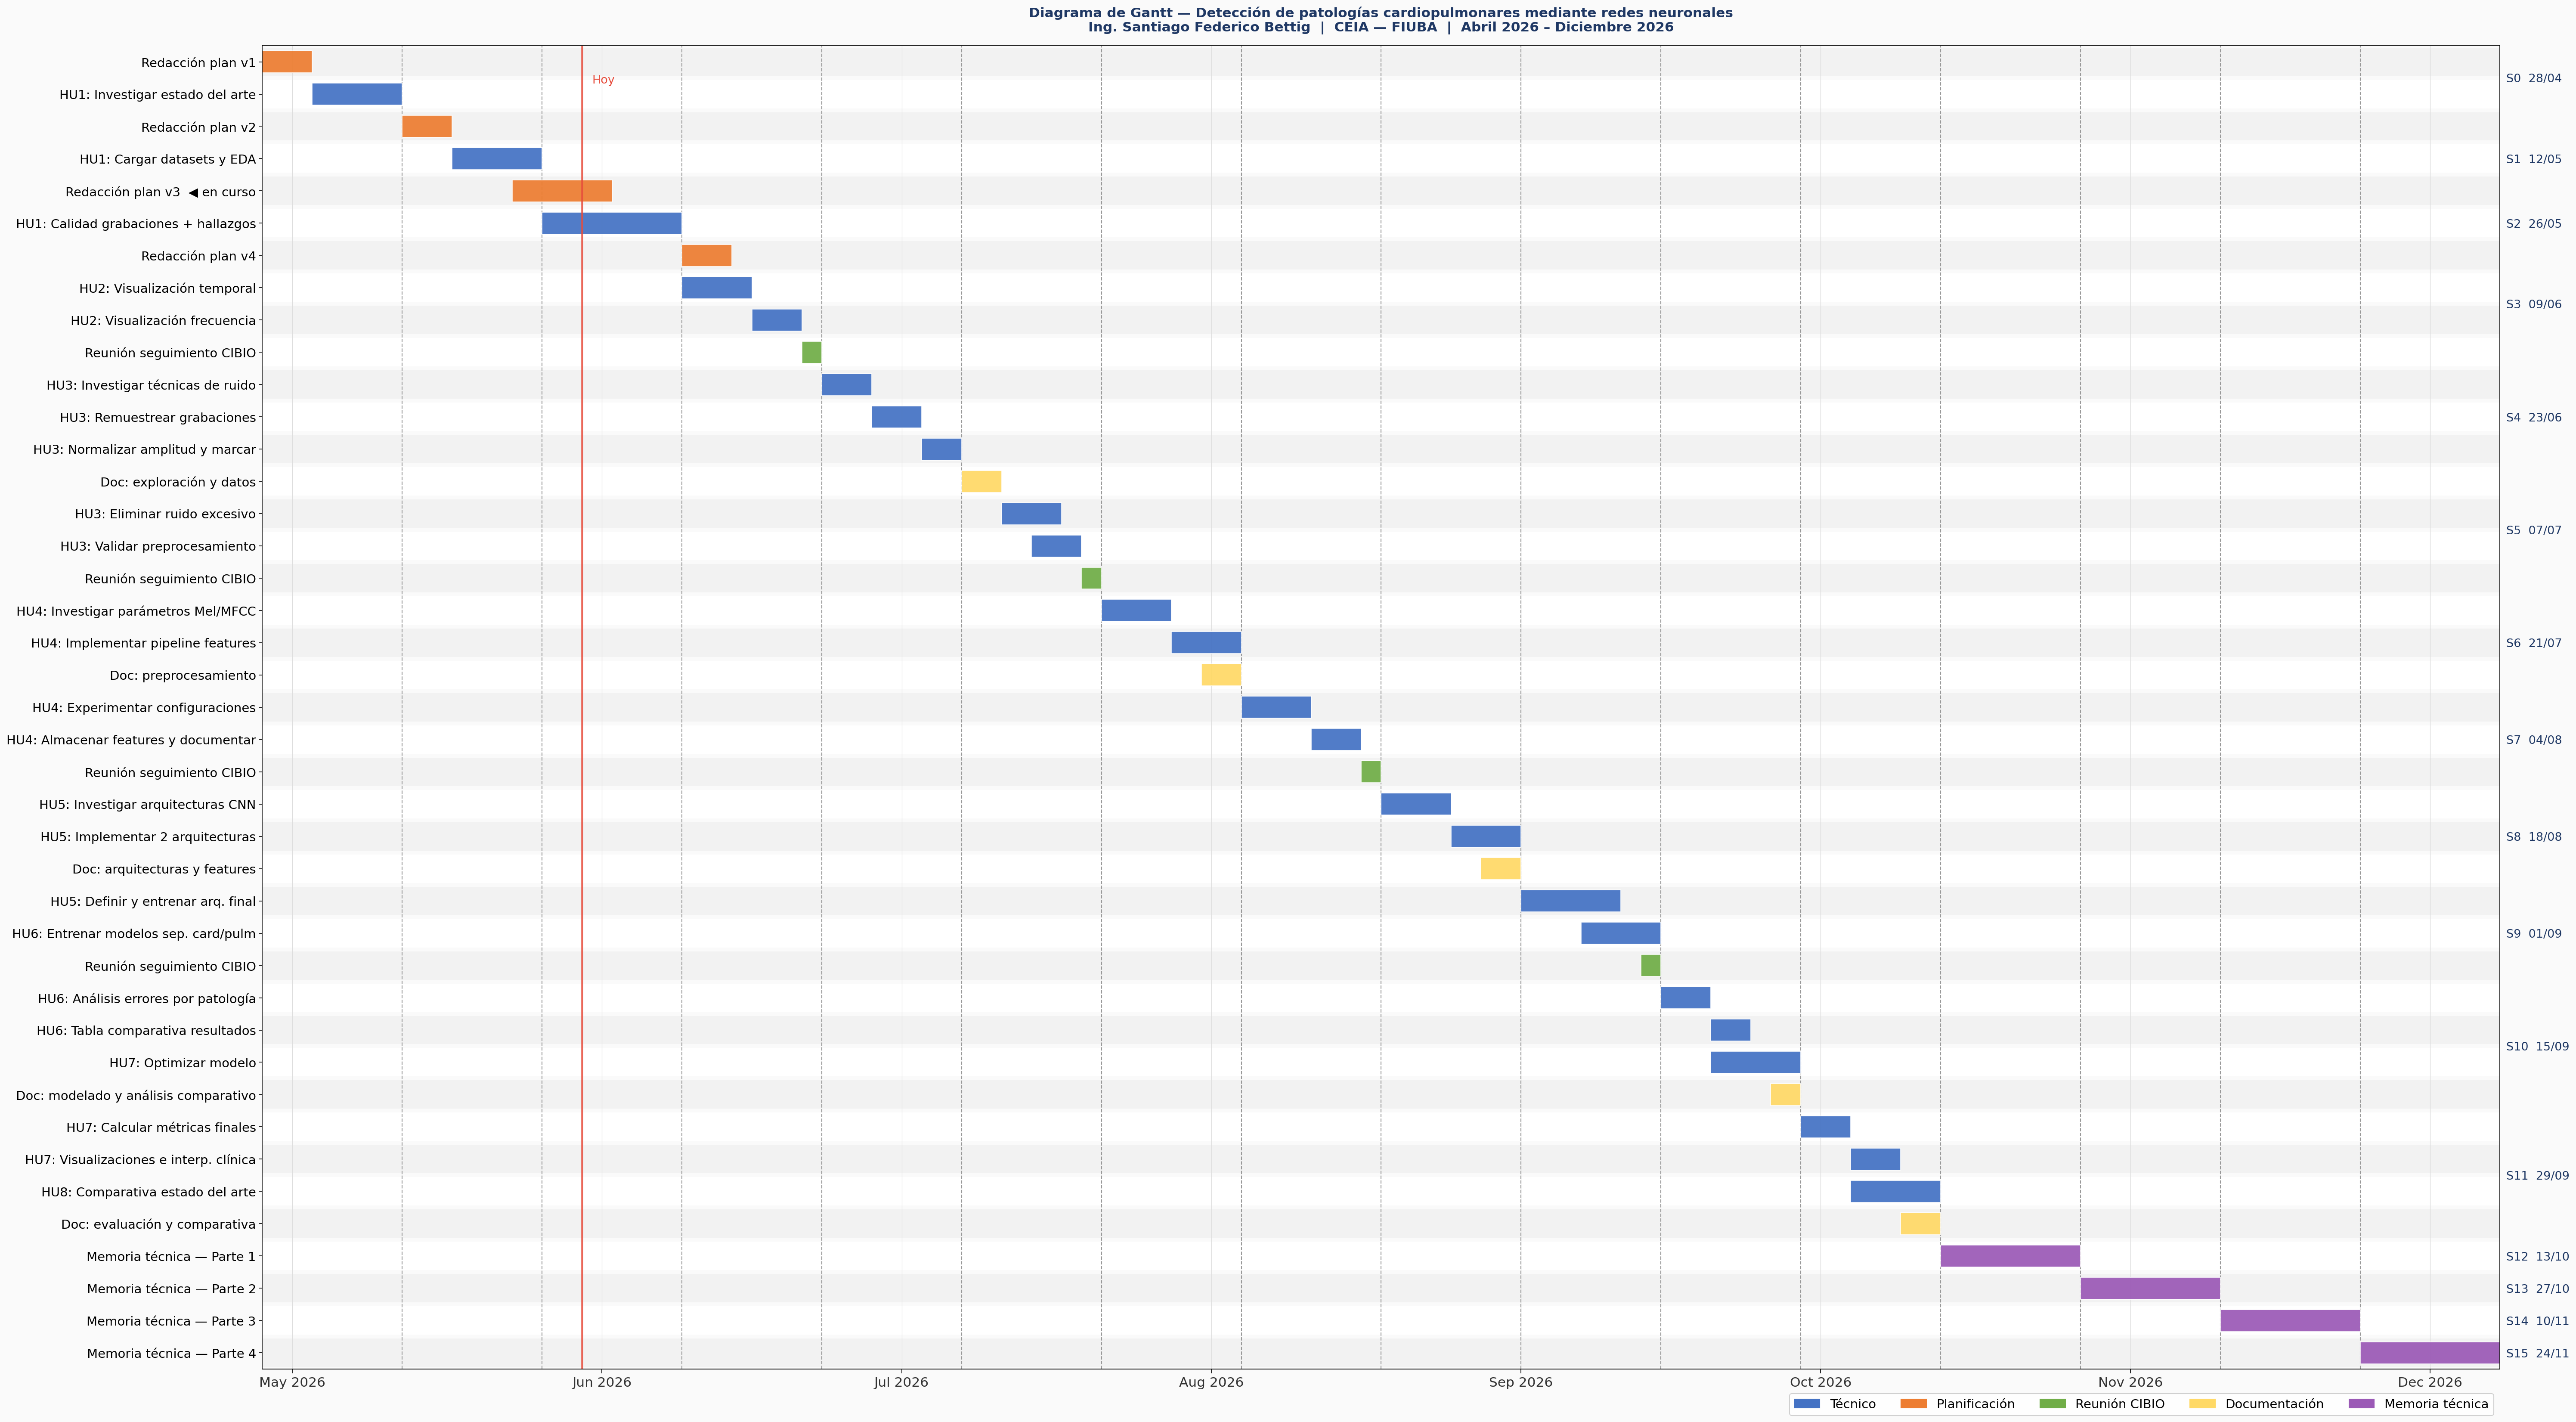
\includegraphics[width=\linewidth, height=\textheight]{./Figuras/gantt_bettig_v7.png}
    \caption{Diagrama de Gantt del proyecto.}
    \label{fig:diagBloques}
\end{figure}
\end{landscape}

\section{12. Gobernanza de datos}
\label{sec:gobernanza}

\subsection{Cumplimiento normativo}

Los datos utilizados en este proyecto provienen de datasets públicos de acceso abierto, los cuales fueron distribuidos libremente 
para investigación y uso académico. Ambos datasets fueron recolectados por sus autores originales, quienes son responsables del cumplimiento normativo en 
dicha etapa. En consecuencia, el presente proyecto no involucra recolección de datos de pacientes reales ni acceso a información 
clínica sensible.

No obstante, dado el carácter biomédico de los datos, corresponde considerar el marco normativo aplicable:
\begin{itemize}
  \item En el plano internacional, el Reglamento General de Protección de Datos (GDPR) de la Unión Europea establece requisitos estrictos 
        para el tratamiento de datos de salud clasificados como datos sensibles. Si bien el proyecto se desarrolla en Argentina y los datos son 
        anónimos, el GDPR es un marco de referencia relevante dado que los datasets provienen de instituciones europeas. 
        En este contexto, el proyecto cumple con sus principios al utilizar datos anónimos, con fines exclusivamente académicos y sin posibilidad 
        de identificación de individuos.
  \item En el plano local, la Ley 25.326 de Protección de los Datos Personales de Argentina regula el tratamiento de datos personales, 
        que incluye los datos de salud como categoría protegida. Dado que los datos utilizados no contienen información que permita 
        identificar a personas físicas, el proyecto se encuadra dentro de los usos permitidos por esta normativa.
  \item En cuanto a la propiedad intelectual, los entregables del proyecto son de carácter académico y de acceso abierto, en línea con lo establecido 
        en el acta de constitución del proyecto. Se respetan las licencias de los datasets originales, que permiten su uso para investigación sin 
        fines comerciales.
\end{itemize}

\subsection{Ética en el uso de la inteligencia artificial}

El desarrollo de sistemas de inteligencia artificial aplicados a la medicina plantea consideraciones éticas que van más allá del cumplimiento normativo estricto. 
Este proyecto adhiere a los principios éticos establecidos por organismos internacionales de referencia, como la UNESCO en su Recomendación 
sobre la Ética de la Inteligencia Artificial (2021) y las guías de la Organización Mundial de la Salud (OMS) para el uso de IA en salud (2021).

Los principios éticos que guían el desarrollo de este trabajo son los siguientes:
\begin{itemize}
  \item Beneficencia y no maleficencia: el sistema está diseñado exclusivamente como herramienta de apoyo al diagnóstico médico. 
        Sus resultados no deben ser interpretados como un diagnóstico definitivo ni reemplazar el criterio clínico del profesional de la salud. 
        Esta limitación está explícitamente incorporada en el propósito y el alcance del proyecto, y deberá ser claramente comunicada en cualquier 
        instancia de uso o difusión del sistema.
  \item Transparencia y explicabilidad: el modelo y su proceso de desarrollo serán documentados de forma completa y reproducible, lo cual permite 
        que otros investigadores puedan auditar, replicar y cuestionar los resultados.
  \item Equidad y no discriminación: los datasets utilizados presentan limitaciones en cuanto a la diversidad de la población representada. 
        Esta limitación será documentada explícitamente y deberá considerarse al momento de evaluar la generalización del modelo a otras poblaciones 
        o contextos clínicos.
  \item Responsabilidad: el responsable del proyecto asume la obligación de garantizar que los resultados sean presentados con rigor académico, 
        sin exagerar las capacidades del sistema ni minimizar sus limitaciones.
  \item Privacidad y protección de datos: aunque los datos utilizados son públicos y anónimos, el proyecto adopta como principio general el 
        tratamiento mínimo y necesario de los datos, para evitar cualquier procesamiento que no sea estrictamente requerido para los objetivos del trabajo.
\end{itemize}

\section{13. Gestión de riesgos}
\label{sec:riesgos}

\subsection{Identificación de riesgos}

Riesgo 1: calidad insuficiente en las grabaciones del dataset. Puede ocurrir que por la variabilidad de las grabaciones, el preprocesamiento no sea 
suficiente y se reduzca la calidad de los datos de entrenamiento.
\begin{itemize}
  \item Severidad(S):4. Un dataset ruidoso o de baja calidad compromete directamente la capacidad de generalización del modelo, lo que puede 
  invalidar los resultados obtenidos.
  \item Probabilidad de ocurrencia(O):3. La literatura indica que los datasets a utilizar son de una calidad aceptable para la investigación, de hecho,
  existen gran cantidad de trabajos relacionados los cuales utilizan estos datos. Por ende, es probable encontrar grabaciones problemáticas, pero no 
  debería ser algo crítico.
\end{itemize}

Riesgo 2: desempeño insuficiente del modelo de clasificación. Puede deberse a una mala elección del alcance o los requisitos, como
también por la calidad insuficiente de los datos (limitaciones del dataset, elección inadecuada de la arquitectura, etc).
\begin{itemize}
  \item Severidad(S):5. Si el modelo tiene un mal desempeño compromete el aporte central del proyecto. Esto puede llevar a un replanteo de las decisiones
  que se tomaron e impactar directo en el cronograma.
  \item Probabilidad de ocurrencia(O):3. El riesgo es inherente a cualquier proyecto de esta índole, podrá ser mitigado con una estrategia acorde.
\end{itemize}

Riesgo 3: el tiempo disponible es menor al planificado. Al desarrollar el proyecto junto a actividades laborales y académicas, existe el riesgo de
que, por circunstancias externas, se reduzca el tiempo disponible por debajo de las 10 h semanales.
\begin{itemize}
  \item Severidad(S):4. Si la disminución de tiempo se sostiene por largos períodos, existirá un impacto directo sobre el cronograma y podría comprometer
  la finalización de las tareas técnicas antes de octubre.
  \item Probabilidad de ocurrencia(O):4. Al desarrollar el proyecto fuera del horario laboral, la probabilidad de que surjan compromisos que reduzcan la
  disponibilidad es alta.
\end{itemize}

Riesgo 4: desbalance severo de las clases en los datasets. Algunos tipos de patologías se presentan mucho más que otras, lo que puede resultar en un modelo
que clasifique a la mayoría como la clase dominante (bajo desempeño).
\begin{itemize}
  \item Severidad(S):4. Si no se corrige el desbalance, puede hacer que el modelo sea inválido, más allá de sus métricas globales.
  \item Probabilidad de ocurrencia(O):4. El desbalance de clases es un problema frecuente, especialmente para patologías poco comunes.
\end{itemize}

Riesgo 5: capacidad de hardware insuficiente para el entrenamiento de modelo. El entrenamiento de este tipo de modelos puede requerir recursos
computacionales significativos.
\begin{itemize}
  \item Severidad(S):3. Que el entrenamiento se haga lento no significa que los resultados sean malos, pero si puede causar retrasos importantes
  en el cronograma.
  \item Probabilidad de ocurrencia(O):2. Los datasets que se van a utilizar no son lo suficientemente grandes como para necesitar una computadora
  con grandes recursos, de ser necesario, existen alternativas como Google Colab que permite el uso de hardware dedicado.
\end{itemize}

\subsection{Tabla de gestión de riesgos}

El RPN (\textit{Risk Priority Number}) se calcula como: $RPN = SxO$. 

Como criterio, se consideran críticos aquellos riesgos cuyo RPN sea superior a 13.

Nota: los valores marcados en la tabla con (*) corresponden a los riesgos una vez mitigados.

\begin{table}[htpb]
\centering
\begin{tabularx}{\linewidth}{@{}|X|c|c|c|c|c|c|@{}}
\hline
\rowcolor[HTML]{C0C0C0} 
Riesgo & S & O & RPN & S* & O* & RPN* \\ \hline
Calidad insuficiente de las grabaciones & 4 & 3 & 12 & - & - & - \\ \hline
Desempeño insuficiente del modelo & 5 & 3 & 15 & 5 & 2 & 10 \\ \hline
Tiempo disponible inferior al planificado & 4 & 4 & 16 & 4 & 2 & 8 \\ \hline
Desbalance severo de clases & 4 & 4 & 16 & 3 & 2 & 6 \\ \hline
Capacidad de hardware insuficiente & 3 & 2 & 6 & - & - & - \\ \hline
\end{tabularx}%
\end{table}

\subsection{Plan de mitigación}

Riesgo 2: desempeño insuficiente del modelo. 
\begin{itemize}
  \item Medidas de mitigación: 
    \begin{itemize}
      \item Adoptar una estrategia de experimentación iterativa desde el primer entrenamiento, junto con una documentación acorde.
      \item Implementar al menos dos arquitecturas candidatas y comparar su desempeño antes de elegir una u otra.
      \item En caso de no alcanzar el requerimiento mínimo, lo primero que debe hacerse es revisar la etapa de extracción de features, ya que
      es la que mas influye sobre el modelo.
    \end{itemize}
  \item Severidad(S*):5. No cambia ya que el potencial impacto sigue presente.
  \item Probabilidad de ocurrencia(O*):2. Se reduce gracias a la estrategia iterativa y a la disponibilidad de técnicas alternativas.
\end{itemize}

Riesgo 3: tiempo disponible inferior al planificado
\begin{itemize}
  \item Medidas de mitigación:
    \begin{itemize}
      \item Incorporar en el cronograma un colchón de contingencia. El último bimestre se reservó para la confección de la memoria técnica y la defensa,
      pero puede usarse para realizar tareas técnicas en paralelo.
      \item Establecer una revisión mensual del avance real vs el planificado y ajustar el alcance si es necesario.
      \item Priorizar las tareas con prioridad alta del backlog y dejar de lado las que tienen prioridad media o baja.
    \end{itemize}
  \item Severidad(S*):4. La severidad no se ve afectada.
  \item Probabilidad de ocurrencia(O*):2. El impacto disminuye gracias al colchón de contingencia y la priorización de las tareas.
\end{itemize}

Riesgo 4: desbalance severo de clases
\begin{itemize}
  \item Medidas de mitigación:
    \begin{itemize}
      \item Darle prioridad al análisis de distribución de clases antes de cualquier decisión sobre el modelado.
      \item Aplicar técnicas de aumentación de datos para incrementar la representación de clases minoritarias.
      \item Utilizar técnicas sensibles al desbalance en lugar de accuracy como criterio principal de evaluación.
    \end{itemize}
  \item Severidad(S*):3. Las métricas adecuadas permiten detectar y corregir el problema a tiempo.
  \item Probabilidad de ocurrencia(O*):2. Disminuye ya que las técnicas de mitigación están bien establecidas en la literatura.
\end{itemize}

\newpage

\section{14. Sprint Review}
\label{sec:sprint_review}
HU2: como desarrollador, quiero visualizar señales de audio representativas de cada patología, para identificar diferencias relevantes 
entre clases y orientar el preprocesamiento de los datos.
\begin{itemize}
  \item Tareas asociadas:
    \begin{itemize}
      \item Tarea 1: graficar la forma de onda temporal de la clases representativas.
      \item Tarea 2: generar representaciones en frecuencia de cada clase y comparar visualmente.
    \end{itemize}
  \item Entregable esperado: gráficos de forma de onda temporal y espectro en frecuencia para al menos dos señales representativas de cada clase.
  \item ¿Cómo sabrás que está cumplida?
    \begin{itemize}
      \item El director verifica que las visualizaciones permitan distinguir diferencias entre clases, como también su correcto etiquetado.
      \item Debe ser posible identificar al menos una diferencia relevante entre clases a partir de los gráficos.
    \end{itemize}
  \item Observaciones o riesgos:
    \begin{itemize}
      \item Que no se identifique ninguna diferencia entre clases.
      \item El cumplimiento depende de la disponibilidad del director.
    \end{itemize}
\end{itemize}

HU4: como desarrollador, quiero extraer las features de cada grabación que me permitan alimentar el modelo.
\begin{itemize}
  \item Tareas asociadas:
    \begin{itemize}
      \item Tarea 1: investigar y comparar parámetros óptimos para espectrogramas Mel y MFCC.
      \item Tarea 2: implementar pipeline para la extracción de datos.
      \item Tarea 3: experimentar con distintas configuraciones de ventana y número de coeficientes.
      \item Tarea 4: validar la calidad de los features generados.
      \item Tarea 5: almacenar los features generados en un formato acorde y documentar lo realizado.
    \end{itemize}
  \item Entregable esperado: ejemplos visuales de espectrogramas Mel y vectores MFCC para cada clase, junto con la documentación de los parámetros utilizados
  y el formato de almacenamiento de los features.
  \item ¿Cómo sabrás que está cumplida?
    \begin{itemize}
      \item Se verifica que los features se hayan generado para todas las grabaciones y que estén almacenados en un formato aceptable.
    \end{itemize}
  \item Observaciones o riesgos:
    \begin{itemize}
      \item Los features no se obtuvieron correctamente y no son suficientes para el debido entrenamiento del modelo.
    \end{itemize}
\end{itemize}

HU5: como desarrollador, quiero diseñar y entrenar un modelo, para clasificar automáticamente los sonidos cardíacos y pulmonares.
\begin{itemize}
  \item Tareas asociadas:
    \begin{itemize}
      \item Tarea 1: investigar arquitecturas aplicables a clasificación de audio médico.
      \item Tarea 2: implementar al menos dos arquitecturas candidatas y comparar.
      \item Tarea 3: definir y documentar la arquitectura del modelo.
      \item Tarea 4: entrenar modelo y ajustar hiperparámetros.
    \end{itemize}
  \item Entregable esperado: modelo entrenado y documentado de manera adecuada.
  \item ¿Cómo sabrás que está cumplida?
    \begin{itemize}
      \item Se evalúa el modelo con un conjunto de audios de prueba.
    \end{itemize}
  \item Observaciones o riesgos:
    \begin{itemize}
      \item Requerimientos computacionales altos.
    \end{itemize}
\end{itemize}

HU7: como desarrollador, quiero evaluar el modelo con métricas estándar (accuracy, F1-score, matriz de confusión), para conocer su capacidad 
de clasificación.
\begin{itemize}
  \item Tareas asociadas:
    \begin{itemize}
      \item Tarea 1: calcular accuracy, F1-score por clase, matriz de confusión y curva ROC sobre el conjunto de prueba.
      \item Tarea 2: generar visualizaciones de cada métrica.
      \item Tarea 3: interpretar resultados en contexto clínico junto al equipo del CIBIO.
      \item Tarea 4: Optimizar modelo luego de obtener los resultados preliminares.
    \end{itemize}
  \item Entregable esperado: tabla comparativa con todas las métricas obtenidas y su debida interpretación.
  \item ¿Cómo sabrás que está cumplida?
    \begin{itemize}
      \item Las métricas deben ser claras y su interpretación no debe permitir ambigüedades. 
    \end{itemize}
  \item Observaciones o riesgos:
    \begin{itemize}
      \item Que los resultados obtenidos no sean suficientes para alcanzar los requerimientos principales.
    \end{itemize}
\end{itemize}

\newpage

\section{15. Sprint Retrospective}    
\label{sec:sprint_retro}

\begin{table}[H]
\renewcommand{\arraystretch}{1.4}
\begin{tabular}{|>{\raggedright\arraybackslash}p{1.8cm}|
                >{\raggedright\arraybackslash}p{2.3cm}|
                >{\raggedright\arraybackslash}p{2.3cm}|
                >{\raggedright\arraybackslash}p{2.3cm}|
                >{\raggedright\arraybackslash}p{2.3cm}|
                >{\raggedright\arraybackslash}p{2.3cm}|}
\hline
\rowcolor[HTML]{CCCCCC} 
\textbf{Sprint tipo y N°} & \textbf{¿Qué hacer más?} & \textbf{¿Qué hacer menos?} & \textbf{¿Qué mantener?} & \textbf{¿Qué empezar a hacer?} & \textbf{¿Qué dejar de hacer?} \\
\hline
Sprint técnico - 4 & Validar visualmente las señales luego de cada paso del preprocesamiento, sin tener el pipeline completo & Iterar indefinidamente sobre la elección de la técnica de eliminación de ruido sin establecer un criterio de corte claro & Documentar de manera incremental cada paso & Comparar las señales antes y después del preprocesamiento desde el inicio  & Postergar validación visual hasta tener el dataset completo preprocesado \\
\hline
Sprint técnico - 8 & Registrar los resultados de cada experimento de forma estructurada para facilitar la comparación entre arquitecturas & Invertir tiempo excesivo en optimizar una arquitectura antes de comparar con otras & Investigar arquitecturas en la literatura antes de diseñar una propia & Monitorear métricas desde el inicio del entrenamiento & Tomar decisiones sobre la arquitectura basadas en la intuición \\
\hline
Sprint técnico - 10 & Analizar errores del modelo para enteder qué clases presentan mayor dificultad & Ajustar hiperparámetros de forma aleatoria & Comparar entre enfoque integrado y por separado & Establecer un criterio de corte para las iteraciones del modelo & Ignorar métricas como fuente de información \\
\hline
Sprint no técnico - 1 & Consultar al director ante dudas sobre el alcance o criterios de evaluación & Extender la etapa de planificación más allá de lo necesario & El registro de cambios del documento & Vincular cada sección del plan con las tareas del backlog & Tratar el plan de proyecto como un documento estático, ya que este es un documento que debe actualizarse constantemente \\
\hline
\end{tabular}
\end{table}

\end{document}